\section{Περιγραφή Λειτουργίας Μονοφασικού Μετατροπέα}

\noindent
Ο μονοφασικός μετατροπέας αποτελεί μία συσκευή η οποία μετατρέπει DC τάση και ρεύμα σε AC. Το κύκλωμα κατασκευάζεται από τέσσερεις ελεγχόμενους διακόπτες και τέσσερεις διόδους συνδεδεμένες ως εξής:
\begin{figure}[H]
	\centering
	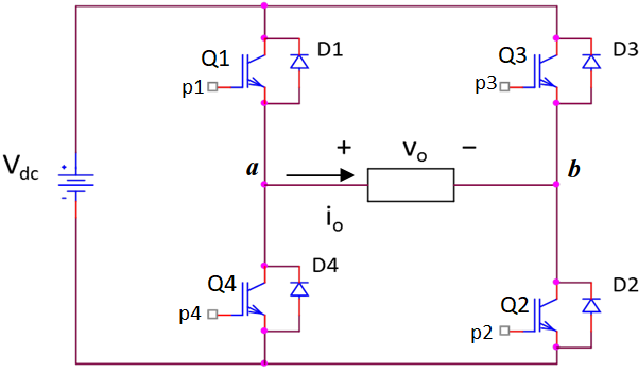
\includegraphics[width=0.45\textwidth]{Images/circuit1.png}
	\label{circuit_1}
\end{figure}

\subsection{Μονοφασικός Αντιστροφέας Γέφυρας Τετραγωνικού Παλμού}
\subsection{Μονοφασικός Αντιστροφέας Γέφυρας με μονοπολική PWM}
\noindent
Για την παραγωγή της εναλλασσόμενης τάσης και εναλλασσόμενου ρεύματος εξόδου, δημιουργούνται τετραγωνικοί παλμοί διαφορετικού μήκους μέσω των οποίων ελέγχεται το πλάτος της τάσης εξόδου, ανάλογα με το μήκος τους.
\noindent\\\\
Για την παραγωγή των παλμών ελέγχου των διακοπτών, κατασκευάζεται το επιθυμητό ημιτονοειδές σήμα καθώς και ένας τριγωνικός παλμός πλάτους $V_{dc}$, συχνότητας ίση με την διακοπτική $(m_f \cdot f)$ και συγκρίνοντας τα δύο σήματα μεταξύ τους προκύπτουν οι αντίστοιχοι παλμοί όπως αυτοί φαίνονται στον πίνακα που ακολουθεί: ΔΕΝ ΕΊΑΝΙ ΤΕΛΕΊΩΣ ΣΩΣΤΌ ΠΡΈΠΕΙ ΝΑ ΔΩ ΤΑ ΔΙΑΓΡΆΜΜΑΤΑ ΓΙΑ ΝΑ ΠΩ ΌΛΕΣ ΤΙΣ ΠΕΡΙΠΤΏΣΕΙΣ